\section{Topics of interest}
Here we discuss in a little more detail the previously outlined topics. These
topics offer us a concise and detailed tests to investigate the programming 
language.

\subsection{Concurrency}
Ada is considered to have a good concurrency support. 

% TODO Revise this part 
\subsection{Sockets}
Sockets are a good topic in this case study, since sockets are OS dependent
therefore will provide some insight on how the language and application will
behave on different platforms. 

\subsection{Cross Platform Filesystem Support}
To programmers that have used languages that do not require virtual machines, 
concerns for cross platform availability of an application, more often arise. 
This case study will use some simple filesystem operations to indicate what we 
may and may not do with the language.

We will investigate how:
\begin{itemize}
  \item Location to resources are handled
  \item Permissions for inodes are handled
\end{itemize}

\subsection{Protocol Implementation}
A topic that I have came accross in programming languages that is somewhat
interesting to see in implementation, are protocols. Notably \textbf{Erlang} 
makes this a breeze. Investigating this in Ada will be interesting. 

For this small project, we'll be implementing 5 parts of the Http protocol. 
Namely the HEAD, GET, POST, PUT and DELETE methods. We refer to the RFC2616 manual \cite{RFC2616}
for the definition of behaviours of these methods. Once they are implemented in
this case study using Ada, the project shall be tested by using any mainstream 
browser such as \textit{Firefox} or \textit{Chromium}.

For the reader we extract the definitions and behaviour of these four methods.
\subsubsection{Overview of Http Protocol}
The Http protocol is a text, request-response protocol. The RFC2616 
specification is quite detailed, but we will be implementing a very 
small subset of the specification for this case study.

The Http version we are concerned with is \textbf{1.1}.

There exists indempodent and non indempodent methods in the Http specification.
GET is described as an indempodent method. That is, if a request is being made
with the same specific set of parameters, then the response should be the same
each time that request is repeated. For example, if we had a function such as
$ f(x) = x + 1 $, then each time we provided $ x = 1 $ we should always retrieve
`2'. We present the following table, which describes the methods we will be 
implementing:
\\
\begin{center}
\begin{tabular}{| c | c |}
\hline
\textbf{Method} & \textbf{Type} \\ \hline \hline
HEAD   & Indempondent \\
GET    & Indempondent \\
POST   & Non-Indempondent \\
PUT    & Indempondent \\ 
DELETE & Indempondent \\
\hline
\end{tabular}
\end{center}
\subsubsection{HEAD}
This Http method requests the header fields of an html document. The message
body is not to be retrieved. Here is an example of what http headers look like.
The definition is taken straight out of the manual: 
\lstinputlisting[language=]{./src/misc/header-definition.txt}

Here is a more practical example. These headers are retrieved from \textit{www.google.ca}:
\lstinputlisting[language=]{./src/misc/html-header.txt}

And this is the expected html response definition from a successful request.
\lstinputlisting[language=]{./src/misc/http-response.txt}

\subsubsection{GET} 
A \textbf{GET} method is defined in the specification, to be used for operations that
require \textbf{reading} information. On the server side, this should not
tamper with the resources. 

A get request requires \textbf{Request-Line} field to be sent. It is up to the
server to look for the resource requested, and send the response afterwards.

Taken directly from the manual, here is a demonstration of what the GET request
looks like, when ``accessing www.w3.org'':
\lstinputlisting[language=]{./src/misc/get-request.txt}

\subsubsection{POST}
\textbf{POST} is the indempodent method we mentioned before. This means each
time a post request is sent, a resource must (usually) be created, always
guaranteeing different response, for a same request.

A more ``hands on'' example of this would be if a user accidentally submited a
form twice by an accidental double click.

\subsubsection{PUT}
We must add more stuff here.

\subsubsection{DELETE} 
We must add more stuff here.

\subsection{First Steps}
The first steps in an Ada application is to define the \textit{project manager 
file} for the given project as outlined on the manual \cite{GNATintro}.

%% TODO: Need to check if this is indeed the case. 
The GNAT project file abstracts a lot of the building details into this file.
It will take care even about other language builds, meaning that if you wish to
create, for example C extensions to the language, you could achieve this
easily, as opposed to tedious makefiles. 

%% TODO
Another added advantage is that GNAT Project Files also take into consideration 
the file naming conventions. Another automated feature in this file is automatic
building of external libraries. There are various other ways to achieve this,
either on a makefile level, or alternatively using features in certain SCM tools
to clone and build the libraries automatically. However having everything in one
file allows for better, quick communication on the specification of ,
albeit coupling very specific 

\subsubsection{Deployment View}
The overall view of the system components can be seen in Figure \ref{fig:deployment}. 

\begin{figure}[hb]
\centering
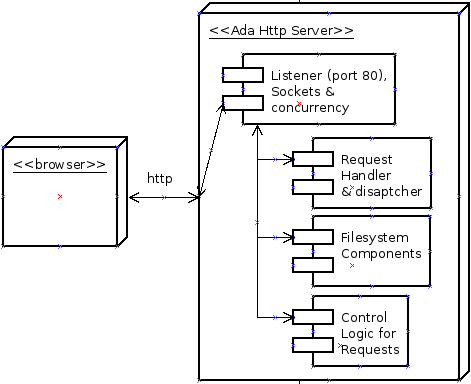
\includegraphics[width=4in]{gfx/deployment.png}
\caption{Deployment Diagram}
\label{fig:deployment}
\end{figure}



